%
% !TEX root = ../../buch.tex
% !TEX encoding = UTF-8
%
%
% teil2.tex -- Der Quadtree-Algorithmus
%
% Schritt für Schritt: Startquadrat, Vierteln, Zählen, Verwerfen, Iterieren.
% Mit der Quadtree-Abbildung (3 Stadien).
%
\section{Der Quadtree-Algorithmus%
\label{weyl:section:algorithmus}}
\rhead{Der Quadtree-Algorithmus}
Mit dem Wegintegral aus Satz~\ref{weyl:satz:nullstellen-zaehlen} können wir nun das
Bisektionsprinzip in die komplexe Ebene übertragen.
Statt eindimensionale Intervalle zu halbieren, vierteln wir zweidimensionale Quadrate und 
statt eines Vorzeichenwechsels prüfen wir das Wegintegral.
Da bei jedem Schritt aus einem Quadrat vier kleinere werden, entsteht eine Baumstruktur,
in der jeder Knoten bis zu vier Kinder hat -- daher der Name \emph{Quadtree}.

\subsection{Das Startquadrat%
\label{weyl:subsection:startquadrat}}
Wir beginnen mit einem Quadrat
\[
D
=
\bigl[-r, r\bigr] \times \bigl[-r, r\bigr]
\subseteq
\mathbb{C}
,
\]
das gross genug gewählt ist, um alle Nullstellen von $f$ zu enthalten.
Aus der Theorie der Polynome ist bekannt, dass für jede Nullstelle $z_k$ von
$f(z) = a_n z^n + \dots + a_0$ die Abschätzung
\[
|z_k|
\leq
\sum_{j=0}^{n-1}
\frac{|a_j|}{|a_n|}
\]
gilt, und damit ist
\begin{equation}
r
=
\sum_{j=0}^{n-1}
\frac{|a_j|}{|a_n|}
\label{weyl:eq:startradius}
\end{equation}
ein zulässiger Wert.
Zur Kontrolle berechnen wir das Wegintegral
$N(D) = \tfrac{1}{2\pi i} \oint_{\partial D} f'/f\, dz$ über das Startquadrat. Das
Resultat muss $N(D) = n$ ergeben, denn alle $n$ Nullstellen liegen drin.
Stimmt diese Probe nicht, hat sich entweder bei der numerischen Integration ein Fehler
eingeschlichen oder eine Nullstelle liegt zufällig auf dem Rand. In beiden Fällen
verschiebt oder vergrössert man $D$ leicht und probiert erneut.

\subsection{Vierteln, Zählen, Verwerfen%
\label{weyl:subsection:vierteln}}
Der iterative Schritt besteht aus drei Teilen.

\subsubsection*{Vierteln}
Ein aktives Quadrat wird durch seine beiden Mittelsenkrechten in vier kongruente
Teilquadrate $D_1, D_2, D_3, D_4$ zerlegt.
Die Kantenlänge halbiert sich dabei in jedem Schritt, die Fläche viertelt sich.
Nach $m$ Iterationen sind die Quadrate auf Kantenlänge $2r/2^m = r/2^{m-1}$
geschrumpft.

\subsubsection*{Zählen}
In jedem Teilquadrat $D_i$ berechnen wir das Wegintegral
\begin{equation}
N(D_i)
=
\frac{1}{2\pi i}
\oint_{\partial D_i}
\frac{f'(z)}{f(z)}
\, dz
.
\label{weyl:eq:teilintegral}
\end{equation}
Dieses Integral ist eine ganze Zahl zwischen $0$ und $n$ und gibt die Anzahl der
Nullstellen im Teilquadrat $D_i$ an.
Als nützliche Probe gilt nach dem Cauchy-Integralsatz, dass sich die vier Werte
zur Nullstellenzahl des Elternquadrats aufsummieren müssen:
\begin{equation}
N(D_1) + N(D_2) + N(D_3) + N(D_4)
=
N(D)
.
\label{weyl:eq:probe}
\end{equation}
Diese Identität ist ein willkommener Selbsttest jeder Iteration.

\subsubsection*{Verwerfen}
Teilquadrate mit $N(D_i) = 0$ enthalten keine Nullstelle und werden aus der weiteren
Betrachtung entfernt.
Alle anderen Teilquadrate werden in einer Liste der aktiven Quadrate gesammelt und
in der nächsten Iteration ihrerseits geviertelt.
Da das Polynom $n$ Nullstellen besitzt, sind höchstens $n$ Teilquadrate gleichzeitig
"voll", sodass die Liste aktiver Quadrate nicht beliebig wächst.

Abbildung~\ref{weyl:fig:quadtree} zeigt das Zusammenspiel der drei Schritte an einem
Beispielpolynom mit acht Nullstellen.

%
% fig/quadtree.tex -- Quadtree-Unterteilung (3 Stadien)
%
% Nachbau der SVG-Abbildung: Startquadrat -> Vierteln & Zaehlen -> Verfeinern
%
\begin{figure}
\centering
\def\weylquadtreezeros{%
  \node[root] at (0.45,3.10) {};
  \node[root] at (1.10,3.10) {};
  \node[root] at (1.45,2.95) {};
  \node[root] at (0.45,2.20) {};
  \node[root] at (3.05,3.10) {};
  \node[root] at (2.10,2.20) {};
  \node[root] at (2.45,2.35) {};
  \node[root] at (1.25,1.20) {};
}
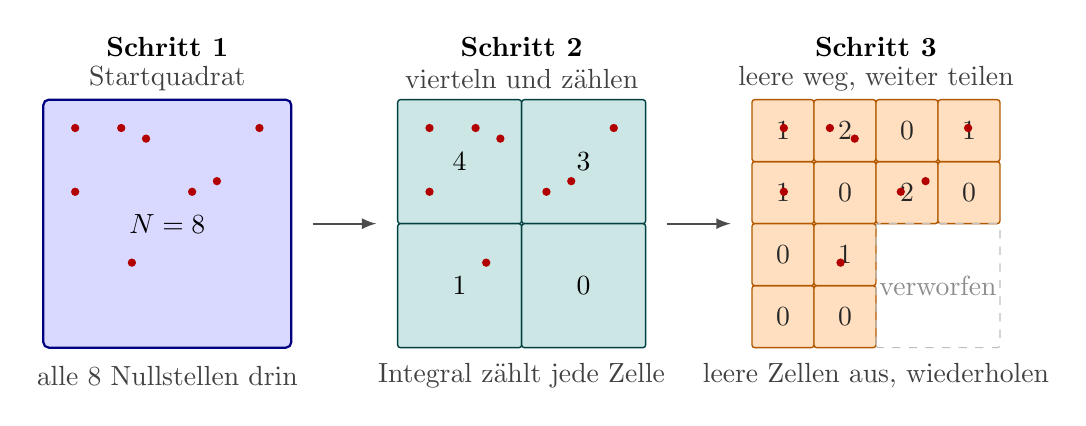
\begin{tikzpicture}[>=latex,thick,
    scale=0.9,
    stage1/.style={fill=blue!15,draw=blue!50!black,line width=0.8pt,rounded corners=2pt},
    stage2/.style={fill=teal!20,draw=teal!50!black,line width=0.5pt,rounded corners=1pt},
    stage3/.style={fill=orange!25,draw=orange!70!black,line width=0.5pt,rounded corners=1pt},
    discarded/.style={draw=gray!50,line width=0.4pt,dashed,rounded corners=1pt},
    root/.style={circle,fill=red!70!black,inner sep=0pt,minimum size=3pt},
    count/.style={font=\bfseries},
    cnt/.style={gray!30!black},
    stagelabel/.style={font=\bfseries},
    sublabel/.style={gray!50!black}]
%
% ============ STADIUM 1: Startquadrat ============
\begin{scope}[xshift=0cm]
  % Stadium-Labels
  \node[stagelabel] at (1.75,4.0) {Schritt 1};
  \node[sublabel] at (1.75,3.55) {Startquadrat};
  \begin{scope}[yshift=-0.25cm]
  % Grosses Quadrat
  \draw[stage1] (0,0) rectangle (3.5,3.5);
  % 8 Nullstellen, konsistent mit den Zählwerten der folgenden Stadien
  \weylquadtreezeros
  % Zentrale Zahl
  \node[count] at (1.75,1.75) {$N = 8$};
  \end{scope}
  % Unter-Beschriftung
  \node[sublabel] at (1.75,-0.65) {alle $8$ Nullstellen drin};
\end{scope}
%
% Pfeil 1
\draw[->,thick,gray!60!black] (3.8,1.5) -- (4.7,1.5);
%
% ============ STADIUM 2: Vierteln und Zählen ============
\begin{scope}[xshift=5cm]
  \node[stagelabel] at (1.75,4.0) {Schritt 2};
  \node[sublabel] at (1.75,3.55) {vierteln und zählen};
  \begin{scope}[yshift=-0.25cm]
  % 4 Quadrate (oben links: 4, oben rechts: 3, unten links: 1, unten rechts: 0)
  \draw[stage2] (0,1.75)    rectangle (1.75,3.5);   % oben links
  \draw[stage2] (1.75,1.75) rectangle (3.5,3.5);    % oben rechts
  \draw[stage2] (0,0)       rectangle (1.75,1.75);  % unten links
  \draw[stage2] (1.75,0)    rectangle (3.5,1.75);   % unten rechts
  % Nullstellen zum Nachzählen
  \weylquadtreezeros
  % Zahlen
  \node[count] at (0.875,2.625) {$4$};
  \node[count] at (2.625,2.625) {$3$};
  \node[count] at (0.875,0.875) {$1$};
  \node[count] at (2.625,0.875) {$0$};
  \end{scope}
  % Unter-Beschriftung
  \node[sublabel] at (1.75,-0.65) {Integral zählt jede Zelle};
\end{scope}
%
% Pfeil 2
\draw[->,thick,gray!60!black] (8.8,1.5) -- (9.7,1.5);
%
% ============ STADIUM 3: Verfeinern, leere weg ============
\begin{scope}[xshift=10cm]
  \node[stagelabel] at (1.75,4.0) {Schritt 3};
  \node[sublabel] at (1.75,3.55) {leere weg, weiter teilen};
  \begin{scope}[yshift=-0.25cm]
  % Oben links (war 4): 4 kleinere Quadrate mit 1 2 1 0
  \draw[stage3] (0,1.75)        rectangle (0.875,2.625);
  \draw[stage3] (0.875,1.75)    rectangle (1.75,2.625);
  \draw[stage3] (0,2.625)       rectangle (0.875,3.5);
  \draw[stage3] (0.875,2.625)   rectangle (1.75,3.5);
  \node[cnt] at (0.4375,3.0625) {$1$};
  \node[cnt] at (1.3125,3.0625) {$2$};
  \node[cnt] at (0.4375,2.1875) {$1$};
  \node[cnt] at (1.3125,2.1875) {$0$};
  % Oben rechts (war 3): 4 kleinere Quadrate mit 0 1 2 0
  \draw[stage3] (1.75,1.75)     rectangle (2.625,2.625);
  \draw[stage3] (2.625,1.75)    rectangle (3.5,2.625);
  \draw[stage3] (1.75,2.625)    rectangle (2.625,3.5);
  \draw[stage3] (2.625,2.625)   rectangle (3.5,3.5);
  \node[cnt] at (2.1875,3.0625) {$0$};
  \node[cnt] at (3.0625,3.0625) {$1$};
  \node[cnt] at (2.1875,2.1875) {$2$};
  \node[cnt] at (3.0625,2.1875) {$0$};
  % Unten links (war 1): 4 kleinere Quadrate mit 0 1 0 0
  \draw[stage3] (0,0)           rectangle (0.875,0.875);
  \draw[stage3] (0.875,0)       rectangle (1.75,0.875);
  \draw[stage3] (0,0.875)       rectangle (0.875,1.75);
  \draw[stage3] (0.875,0.875)   rectangle (1.75,1.75);
  \node[cnt] at (0.4375,1.3125) {$0$};
  \node[cnt] at (1.3125,1.3125) {$1$};
  \node[cnt] at (0.4375,0.4375) {$0$};
  \node[cnt] at (1.3125,0.4375) {$0$};
  % Unten rechts (war 0): verworfen, gestrichelt
  \draw[discarded] (1.75,0) rectangle (3.5,1.75);
  % Nullstellen zum Nachzählen
  \weylquadtreezeros
  \node[sublabel,opacity=0.6] at (2.625,0.875) {verworfen};
  \end{scope}
  % Unter-Beschriftung
  \node[sublabel] at (1.75,-0.65) {leere Zellen aus, wiederholen};
\end{scope}
%
\end{tikzpicture}
\caption{Drei Stadien von Weyls Algorithmus an einem Beispielpolynom mit $8$ Nullstellen.
Links das Startquadrat $D = [-r,r] \times [-r,r]$, das alle Nullstellen umschliesst.
Mitte: nach der ersten Iteration ist $D$ in vier Teilquadrate zerlegt, das
Wegintegral liefert die Nullstellenanzahl jedes Teilquadrats; in unserem Beispiel
$4$, $3$, $1$ und $0$ --- die Probe $4+3+1+0 = 8$ stimmt.
Rechts: das leere Quadrat (unten rechts) wird verworfen, die übrigen drei werden
ihrerseits geviertelt. Der Prozess wiederholt sich, bis jede Nullstelle in einem
eigenen kleinen Quadrat isoliert ist.
\label{weyl:fig:quadtree}}
\end{figure}


\subsection{Abbruch und Übergabe%
\label{weyl:subsection:abbruch}}
Die Iteration läuft so lange, bis jede Nullstelle in einem eigenen Quadrat isoliert
ist, also bis für jedes aktive Quadrat $N(D_i) = 1$ gilt und die Kantenlänge unter eine
vorgegebene Schranke $\varepsilon > 0$ gefallen ist.
An diesem Punkt liefert der Quadtree für jede Nullstelle einen kleinen rechteckigen
Suchbereich, dessen Mittelpunkt eine gute Näherung darstellt.

Wie viele Iterationen sind nötig?
Die Kantenlänge halbiert sich pro Schritt, die Genauigkeit verdoppelt sich also
pro Runde, genau wie bei der reellen Bisektion.
Um auf $\varepsilon$-Genauigkeit zu kommen, braucht man etwa
$m \approx \log_2(2r/\varepsilon)$ Iterationen.
Für eine Genauigkeit von $10^{-6}$ bei Startradius $r = 10$ sind das rund $24$ Schritte.

\subsection{Pseudocode%
\label{weyl:subsection:pseudocode}}
Stellen wir die Schritte als kompakten Pseudocode zusammen.
Listing~\ref{weyl:alg:quadtree} fasst den Algorithmus zusammen.

\begin{algorithm}[!h]
\caption{Weyls Quadtree-Algorithmus\label{weyl:alg:quadtree}}
\begin{algorithmic}[1]
\Require Polynom $f$ vom Grad $n$, Genauigkeit $\varepsilon > 0$
\Ensure Liste von Quadraten, die je eine Nullstelle enthalten
\State Wähle Startradius $r$ gemäss \eqref{weyl:eq:startradius}
\State Setze $D_0 \gets [-r,r] \times [-r,r]$
\State $\mathcal{A} \gets \{D_0\}$
  \Comment{Liste aktiver Quadrate}
\State $\mathcal{R} \gets \emptyset$
  \Comment{Liste isolierter Nullstellen}
\While{$\mathcal{A} \neq \emptyset$}
  \State Entnimm ein Quadrat $D$ aus $\mathcal{A}$
  \State Viertle $D$ in $D_1, D_2, D_3, D_4$
  \ForAll{$i = 1, \dots, 4$}
    \State Berechne $N(D_i) = \frac{1}{2\pi i} \oint_{\partial D_i} \frac{f'}{f}\, dz$
    \If{$N(D_i) = 0$}
      \State verwerfe $D_i$
    \ElsIf{$N(D_i) = 1$ und Kantenlänge von $D_i$ $< \varepsilon$}
      \State füge $D_i$ zu $\mathcal{R}$ hinzu
    \Else
      \State füge $D_i$ zu $\mathcal{A}$ hinzu
    \EndIf
  \EndFor
\EndWhile
\State \Return $\mathcal{R}$
\end{algorithmic}
\end{algorithm}

Die einzige nicht-triviale Operation ist die Auswertung des Wegintegrals, die nach
Belieben numerisch (z.\,B. mit der Mittelpunktregel oder einem adaptiven Verfahren) oder
algebraisch (über euklidische Polynomdivision, vgl. Sturm-Folgen) durchgeführt werden
kann \cite{weyl:eisermann}.
Da der Integrand $f'/f$ rational ist und das Resultat eine ganze Zahl sein muss, genügt
schon eine moderate numerische Genauigkeit. Ein Fehler kleiner als $\tfrac{1}{2}$
identifiziert die korrekte ganze Zahl eindeutig.

\subsection{Ein durchgerechnetes Beispiel%
\label{weyl:subsection:beispiel}}
Wir illustrieren den Algorithmus am Polynom
\begin{equation}
f(z)
=
z^3 - 2z + 2
,
\label{weyl:eq:beispiel-polynom}
\end{equation}
mit Ableitung $f'(z) = 3z^2 - 2$.
Die exakten Nullstellen lassen sich noch mit der Formel von Cardano berechnen und
lauten näherungsweise
\[
z_1 \approx -1{,}7693
,
\qquad
z_{2,3} \approx 0{,}8846 \pm 0{,}5897\,i
.
\]
Wir tun aber so, als kennen wir sie nicht, und lassen den Algorithmus arbeiten.

\subsubsection*{Startquadrat}
Mit den Koeffizienten $a_0 = 2$, $a_1 = -2$, $a_2 = 0$, $a_3 = 1$ liefert die Formel
\eqref{weyl:eq:startradius}
\[
r
=
\frac{|a_0| + |a_1| + |a_2|}{|a_3|}
=
\frac{2 + 2 + 0}{1}
=
4
,
\]
also $D_0 = [-4, 4] \times [-4, 4]$ als Startquadrat.
Die numerische Auswertung von $\frac{1}{2\pi i} \oint_{\partial D_0} f'/f \, dz$
mittels Mittelpunktregel auf jeder Seite ergibt den Wert $3$, in Übereinstimmung
mit dem Grad des Polynoms.

\subsubsection*{Erste Iteration}
Vierteln von $D_0$ liefert die vier Teilquadrate
\[
D_1 = [-4, 0] \times [\,0, 4\,]
,
\quad
D_2 = [\,0, 4\,] \times [\,0, 4\,]
,
\quad
D_3 = [-4, 0] \times [-4, 0]
,
\quad
D_4 = [\,0, 4\,] \times [-4, 0]
.
\]
Die Auswertung der Wegintegrale liefert allerdings nichtganzzahlige Werte:
$N(D_1) \approx 0{,}5 - 1{,}01\,i$ und $N(D_3) \approx 0{,}5 + 1{,}01\,i$.
Das ist kein Rechenfehler, sondern die Symptomatik des in
Abschnitt~\ref{weyl:subsection:mehrfache} angesprochenen Sonderfalls. Die reelle
Nullstelle $z_1 \approx -1{,}7693$ liegt exakt auf dem Rand $y = 0$ zwischen $D_1$
und $D_3$.
Wir verschieben das Gitter um einen kleinen Betrag $\delta = 10^{-2}$ und teilen
stattdessen bei der waagerechten Linie $y = \delta$.
Mit dieser Korrektur ergibt die erste Iteration
\begin{center}
\begin{tabular}{lc}
\toprule
Teilquadrat & $N$ \\
\midrule
$D_1' = [-4, 0] \times [\delta, 4]$ & $0$ \\
$D_2' = [\,0, 4\,] \times [\delta, 4]$ & $1$ \\
$D_3' = [-4, 0] \times [-4, \delta]$ & $1$ \\
$D_4' = [\,0, 4\,] \times [-4, \delta]$ & $1$ \\
\midrule
Summe & $3$ \\
\bottomrule
\end{tabular}
\end{center}
Die Probe stimmt, und $D_1'$ wird als nullstellenfrei verworfen.
Schon nach einer Iteration sind die drei Nullstellen voneinander getrennt.

\subsubsection*{Weitere Iterationen}
Wir konzentrieren uns auf $D_2'$, das die Nullstelle $z_2 \approx 0{,}8846 + 0{,}5897\,i$
enthält.
Vierteln liefert vier Teilquadrate, von denen drei leer sind und nur das
Quadrat $[0, 2] \times [\delta, 2{,}005]$ den Wert $N = 1$ liefert.
Eine weitere Vierteln-Runde isoliert die Nullstelle im Quadrat
$[0, 1] \times [\delta, 1{,}008]$ mit Kantenlänge $\approx 1$.
Wir setzen das Verfahren noch so lange fort, bis die Kantenlänge unter $\varepsilon$
fällt, und übergeben dann den Mittelpunkt an das Newton-Verfahren.

\subsubsection*{Übergabe an Newton}
Brechen wir bereits nach der ersten Vierteln-Runde innerhalb von $D_2'$ ab und
nehmen den groben Mittelpunkt $\hat z = 1 + i$ als Startwert für die Newton-Iteration
\[
z_{k+1}
=
z_k
-
\frac{z_k^3 - 2 z_k + 2}{3 z_k^2 - 2}
,
\]
so erhalten wir
\begin{center}
\begin{tabular}{rll}
\toprule
$k$ & $z_k$ & $|z_k - z_2|$ \\
\midrule
$0$ & $1{,}0000 + 1{,}0000\,i$ & $4{,}3 \cdot 10^{-1}$ \\
$1$ & $0{,}9000 + 0{,}7000\,i$ & $1{,}1 \cdot 10^{-1}$ \\
$2$ & $0{,}8837 + 0{,}6003\,i$ & $1{,}1 \cdot 10^{-2}$ \\
$3$ & $0{,}8846 + 0{,}5898\,i$ & $1{,}1 \cdot 10^{-4}$ \\
$4$ & $0{,}8846461653 + 0{,}5897428062\,i$ & $1{,}2 \cdot 10^{-8}$ \\
$5$ & $0{,}8846461771 + 0{,}5897428050\,i$ & $< 10^{-10}$ \\
\bottomrule
\end{tabular}
\end{center}
Die quadratische Konvergenz ist gut zu erkennen. Die Anzahl korrekter Nachkommastellen
verdoppelt sich von Schritt zu Schritt und nach fünf Iterationen ist die
Maschinengenauigkeit nahezu erreicht.
Für $z_3 = \overline{z_2}$ und $z_1$ verläuft das Verfahren analog mit jeweils
eigenem Startquadrat.

Dieses kleine Beispiel illustriert die Hauptpunkte des Algorithmus auf engem Raum.
Die Probe \eqref{weyl:eq:probe} fängt einen Rand-Sonderfall ab, der Quadtree trennt
die drei Nullstellen schon innerhalb weniger Iterationen und das Newton-Verfahren
übernimmt für die Feinkonvergenz die letzten Dezimalstellen in wenigen Schritten.

\subsection{Mehrfache Nullstellen und Sonderfälle%
\label{weyl:subsection:mehrfache}}
Liegen mehrere Nullstellen sehr nah beieinander oder fällt eine mehrfache Nullstelle
in ein Quadrat, so bleibt $N(D_i) \geq 2$, auch wenn das Quadrat schon klein ist.
Der Algorithmus erkennt das automatisch und teilt weiter, bis sich die Nullstellen
trennen oder das Quadrat so klein wird, dass man die Nullstellen als praktisch
zusammenfallend betrachten kann.
Liegt eine echte mehrfache Nullstelle vor, terminiert das Verfahren erst wenn die
Kantenlänge unter $\varepsilon$ fällt. Das Quadrat mit $N(D_i) = k > 1$ wird dann mit
dem Hinweis {$k$-fache Nullstelle} ausgegeben.

Liegt zufällig eine Nullstelle exakt auf dem Rand $\partial D_i$ eines Quadrats, so ist
das Integral nicht wohldefiniert.
In der Praxis verschiebt man dann die Gitterlinien um einen kleinen Betrag oder
verwendet ein leicht verschobenes Startquadrat. Da es nur endlich viele Nullstellen
gibt, lässt sich diese Situation immer vermeiden.
